
Current trends in the software development for the numerical solving of Partial Differential Equations (PDEs), 
and here in particular for Finite Element (FEM) approaches, 
go clearly towards object oriented techniques and adaptive methods in any sense. 
Hereby the employed data and solver structures, and especially the matrix structures, are often in contradiction to modern hardware platforms. As a result, the observed computational efficiency is far 
away from expected peak rates of several GFLOP/s nowadays, and the "real life" gap will even further 
increase. Since high performance calculations 
may be only reached by explicitly 
exploiting "caching in" and "pipelining" in combination with sequentially stored
arrays (using special machine optimised linear algebra libraries), the corresponding 
realisation seems to be "easier" for simple Finite Difference approaches. So, the question arises 
how to perform similar techniques for much more sophisticated Finite Element codes.

These discrepancies between modern mathematical approaches and computational 
demands for highly structured data often lead to unreasonable calculation times for "real world" problems, 
e.g.\ {\em Computational Fluid Dynamics} (CFD) calculations in 3D, as can be seen from recent benchmarks
\cite{TurekSchaeferRannacher1998} for commercial as well as research codes. Hence, strategies for efficiency enhancement
are necessary, not only from the mathematical (algorithms, discretisations) 
but also from the software point of view.
To realise some of the aformentioned necessary improvements, we develope the new Finite Element package 
({\bf FEAST} 
-- {\bf F}inite {\bf E}lement {\bf A}nalysis \& {\bf S}olution {\bf T}ools). 
This package is based on the following concepts:

\begin{itemize}
\item (recursive) "Divide and Conquer" strategies,
\item hierarchical data, solver and matrix structures,
\item {\sc ScaRC} as generalization of multigrid and domain decomposition techniques,
\item frequent use of machine optimised linear algebra routines, 
\item all typical Finite Element facilities included.
\end{itemize}
%
%
The result is a flexible software package with special emphasis on:
%
\begin{itemize}
\item (closer to) peak performance on modern processors,
\item typical multigrid behaviour w.r.t.\ efficiency and robustness,
\item parallelisation tools directly included on low level,
\item open for different adaptivity concepts ($r$- and $h$-adaptivity),
\item low storage requirements, 
\item application to many "real life" problems possible.
\end{itemize}

\noindent
Figure \ref{skizze} shows the general structure of the FEAST package:

\begin{figure}[!h]
\begin{center}
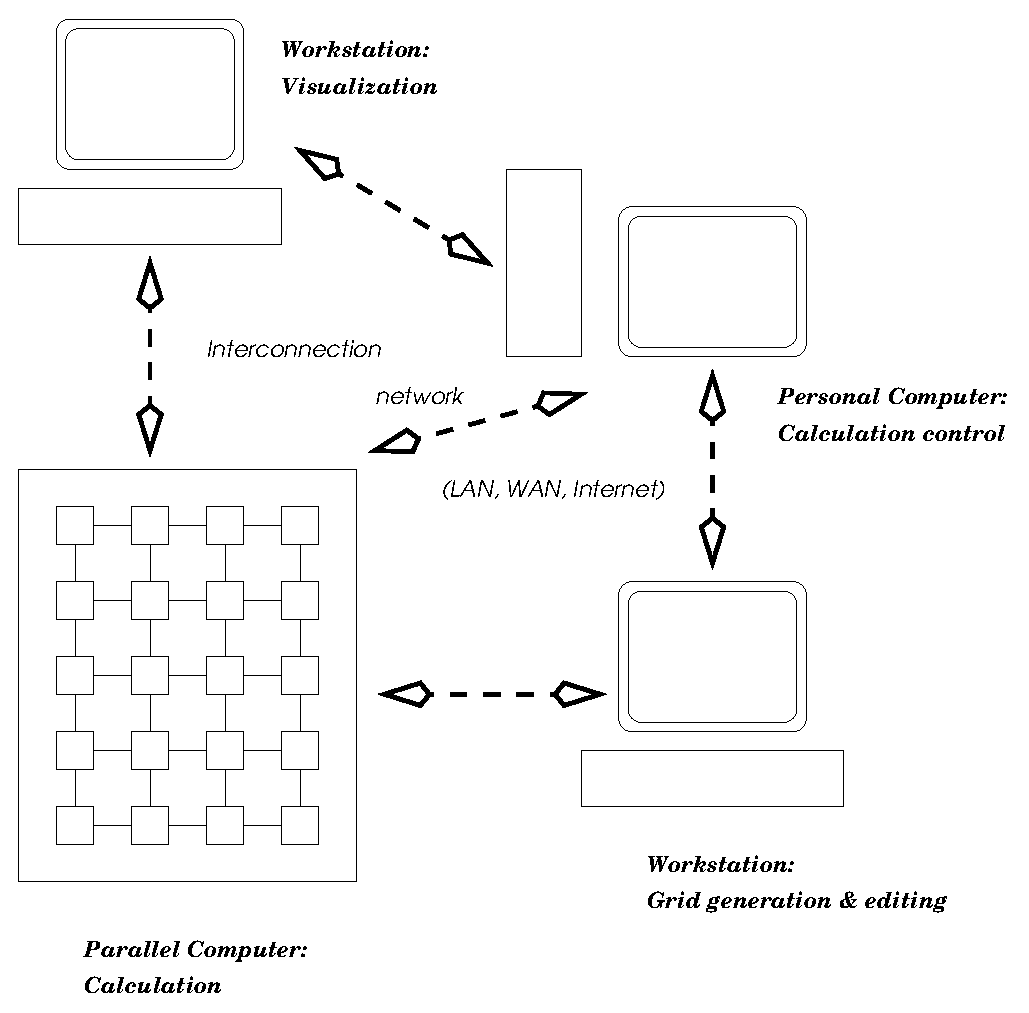
\includegraphics[scale=0.3]{../psfiles/net.eps}\hspace*{1cm}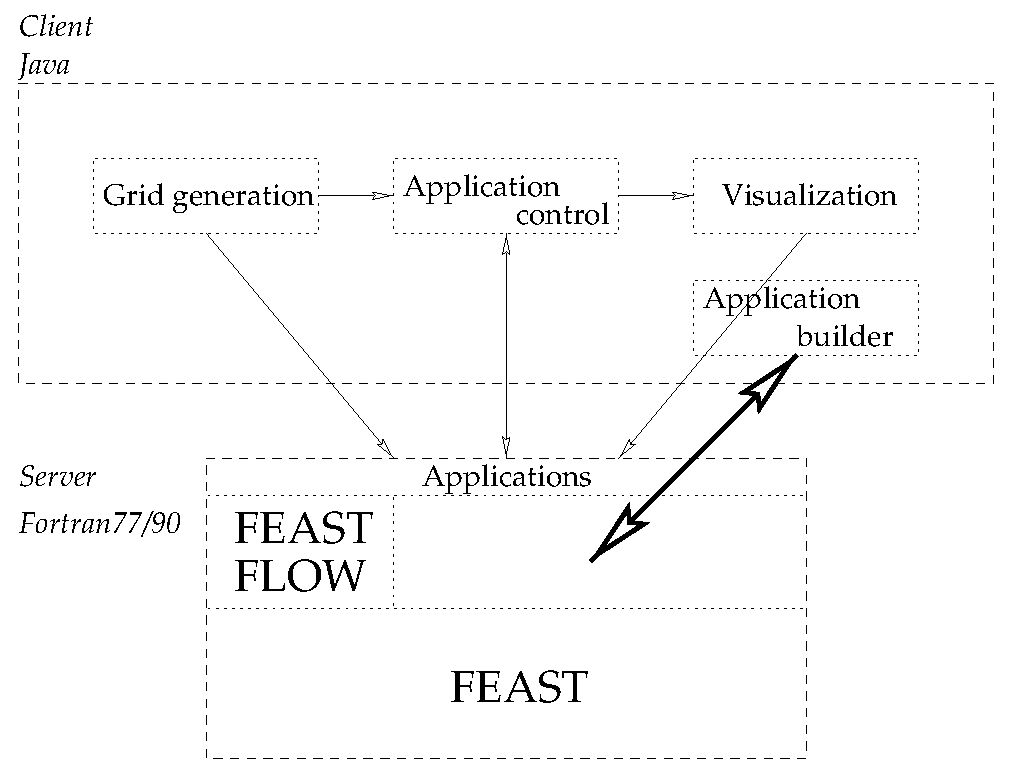
\includegraphics[scale=0.34]{../psfiles/skizze.eps}
\end{center}
\label{skizze}
\caption{FEAST structure and configuration}
\end{figure}

As programming language Fortran (77 and 90) is used. The explicit use of the
two Fortran dialects arises from following observations. For Fortran77 very
efficient and well tried compilers are available which allow to exploit much of the machine performance. 
Furthermore, it is possible
to reuse many reliable parts of the predecessor packages FEAT2D, FEAT3D
and FEATFLOW \cite{TurekBecker1999}. On the other hand Fortran77 is not more than
a better "macro assembler", the very limited language constructs
make the project work very hard. In addtition to that, F77 is no longer the current standard,
so support of this language will stop in near future. And which developer can be
motivated to program in F77?

F90 on the other hand is the new standard and provides new helpful features like records, dynamic memory 
allocation, etc. But there are several disadvantages. The language is very overloaded and the realisation
of some features like pointers is not succeeded. More severe, the compilers for Fortran 90 have not reached
the amount of stability and robustness yet like their Fortran 77 counterparts.  

The compromise is to implement the time critical routines from the numerical
linear algebra in F77, while the administrative routines are based on F90.

The pre-- and postprocessing is mainly handled by Java based program parts. 
Configuring a high performance computer as a FEAST server, the user shall be able to perform the 
remote calculation by a FEAST client. 
 

%#####################################################################



In the following we give examples for "real" computational efficiency results of typical 
numerical tools which help to motivate our hierarchical data, solver and 
matrix structures. For a better understanding, we illustrate shortly in the subsequent chapter the 
corresponding solution technique {\sc ScaRC} ({\bf Sca}lable {\bf R}ecursive {\bf C}lustering) in 
combination with the overall "Divide and Conquer" philosophy. This solver concept forms an essential part
of {\sc FEAST}. 
We discuss how typical multigrid rates can be achieved on parallel 
as well as sequential computers with a very high computational efficiency.

The typical situation in high performance computing today shows the following situation:


{\bf Example}: STAR-CD ($k-\epsilon$), 500 000 cells (by Daimer Chrysler),
SGI Origin2000 (6 CPUs), 6.5 CPU h

\begin{table}[!h]
\begin{center}
\begin{tabular}{|c||c|c||c|} \hline
{\bf Quantity}     & {\bf Experiment}  & {\bf Simulation}& {\bf Difference}\\ \hline
%
Drag (`$c_w$') & 0.165 & 0.317& {\bf 92 \%} \\
Lift (`$c_a$')   & -0.083 & -0.127& {\bf 53 \%} \\ \hline
\end{tabular}
\end{center}
\caption{Star-CD Experiment and Simulation}
\end{table}


\begin{figure}[!h]
\begin{center}
\begin{rotate}{270}
\includegraphics[scale=0.3]{../psfiles/sae.eps.0}
\end{rotate}
\hspace*{7.25cm}\begin{turn}{270}
 \includegraphics[scale=0.3]{../psfiles/sae.eps.1}
\end{turn}
\end{center}
\caption{Star-CD Simulation}
\end{figure}


%#####################################################################




\section{Main Principles in FEAST}

\subsection{Hierarchical data, solver and matrix structures}


One of the most important principles in {\sc FEAST} is to apply consequently a 
{\it (Recursive) Divide and Conquer} strategy. The solution of the complete "global" problem is recursively 
split into smaller "independent" subproblems on "patches" as part of the complete set of unknowns. 
Thus the two major aims in this splitting procedure which can be performed by hand or via self--adaptive 
strategies are:

\begin{itemize}
\item {\em Find locally structured parts.}
\item {\em Find locally anisotropic parts.}
\end{itemize}

Based on "small" structured subdomains on the lowest level (in fact, even one single or a small number of 
elements is allowed), the "higher--level" substructures are generated via clustering of "lower--level" 
parts such that algebraic or 
geometric irregularities are hidden inside the new "higher-level" patch. Additional background information
on this strategy is given in the following sections which describe the corresponding 
solvers related to each stage.

Figures \ref{FIG_f1s} and \ref{FIG_f2s} illustrate exemplarily the employed data structure for a (coarse) triangulation of a 
given domain and its recursive partitioning into several kinds of substructures.

\begin{figure}[htbp]
\begin{center}
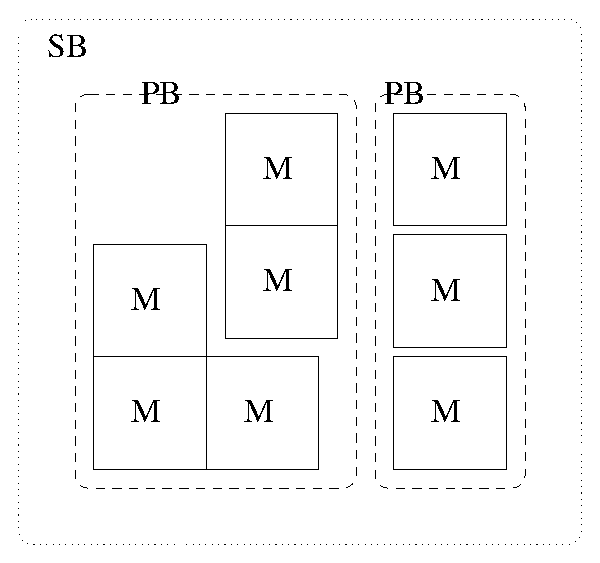
\includegraphics[scale=0.4]{../psfiles/ds1.eps} \hspace*{1cm} 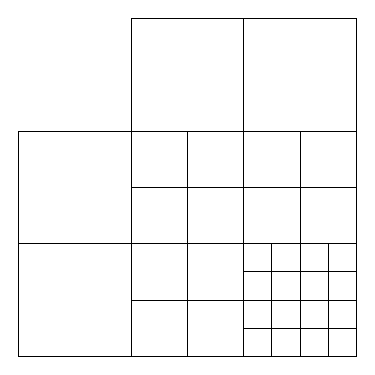
\includegraphics[scale=0.6]{../psfiles/ds2.eps}
\end{center}
\caption{FEAST domain structure}
\label{FIG_f1s}
\end{figure}

According to this decomposition, a corresponding data tree -- the skeleton of the partitioning strategy 
-- describes the hierarchical decomposition process. It consists of a specific collection of elements, 
macros, matrix blocks (MB), parallel blocks (PB), subdomain blocks (SB), etc.

\begin{figure}[htbp]
\begin{center}
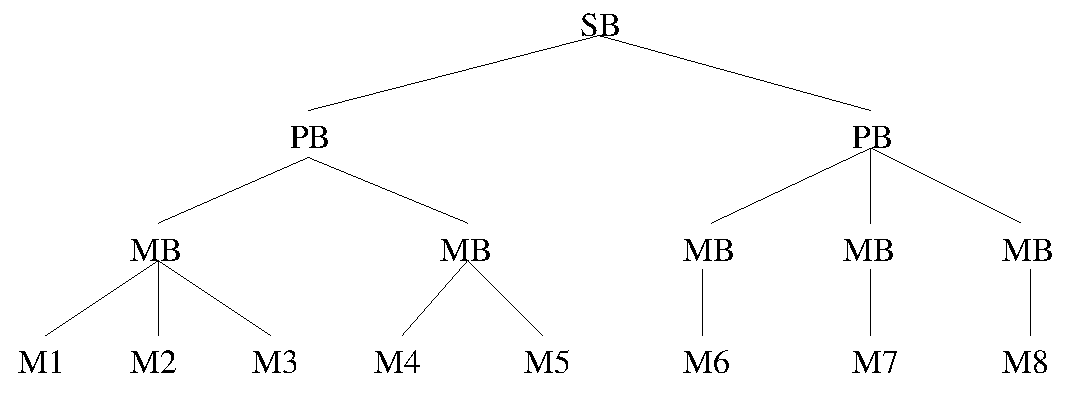
\includegraphics[scale=0.4]{../psfiles/baum.eps}
\end{center}
\caption{FEAST data tree}
\label{FIG_f2s}
\end{figure}

The {\em atomic units} in our decomposition are the "macros" which may be of type {\bf structured} 
(as $n \times n$ collection of quadrilaterals (in 2D) with local band matrices) or 
{\bf unstructured} (any collection of elements, for instance in the case of fully adaptive local grid 
refinement). These "macros" (one or several) can be clustered to build a "matrix block" which 
contains the "local matrix parts": only here is the complete matrix information stored.
Higher level constructs are "parallel blocks" (for the parallel distribution and the realisation of the load balancing) and "subdomain blocks" 
(with special conformity rules with respect to grid refinement and applied discretisation spaces). 
They all together build the complete domain, resp. the complete set of unknowns. It is important to realise 
that each stage in this hierarchical tree can act as independent "father" in relation to its 
"child" substructures. At the same time, it can act as a "child" another phase of the solution 
process (inside of the {\sc ScaRC} solver, see below).

According to this data structure and with respect to the following solver engine
Scarc in FEAST every vector belongs to one hierachical layer Subdomain (SD), Parallelblock (PB) 
and Matrixblock (MB). This concerns the way of data exchange and synchronisation.
If you e.g. perform an exchange operation to a PB-vector, then the vector is modified only
on the PB boundaries to have the same values, but not on the outer boundaries.

\subsection{Generalised solver strategy {\sc ScaRC}}

In short form our long time experience with the numerical and computational runtime behaviour of typical 
multigrid (MG) and Domain Decomposition (DD) solvers can be concluded as follows:

\subsubsection{Some observations from standard multigrid approaches:}

While in fact the numerical convergence behaviour of (optimised) multigrid is very satisfying with 
respect to robustness and efficiency requirements, there still remain some "open" problems: often 
the parallelisation of powerful recursive smoothers (like SOR or ILU) leads to performance degradations 
since they can be realised only in a blockwise sense. Thus it is often not clear how the nice 
numerical behaviour in sequential codes for complicated geometric structures or local anisotropies can be 
reached in parallel computations. And additionally, the communication overhead especially on 
coarser grid levels dominates the total CPU time.
Even more important is the "computational observation" that the 
realised performance on modern platforms is often far beyond (sometimes less than 1 \%) the expected 
peak performance. Many codes often reach much less than 50 MFLOP/s, and this on computers which are said 
(by the vendors) to run with several GFLOP/s peak performance. The reason is simply that 
the single components in multigrid (smoother, defect calculation, grid transfer) perform too few 
arithmetic work with respect to each data exchange such that the facilities of modern superscalar 
architectures are poorly exploitable. In contrast,  we will show that in fact 30 -- 70 \% 
are within reach with appropriate techniques.

\subsubsection{Some observations from standard Domain Decomposition approaches:}


In contrast to standard multigrid, the parallel efficiency is much higher, at least as long as 
no large overlap region between processors must be exchanged. While {\em overlapping} DD methods do not require additional coarse grid problems (however the implementation in 3D for complicated domains or 
for complex Finite Element spaces is a hard job), {\em non-overlapping} DD approaches require 
certain coarse grid problems, as the BPS preconditioner for instance which may lead again to several 
numerical and 
computational problems, depending on the geometrical structure or the used discretisation spaces. 
However the most important difference between Domain Decomposition and multigrid are the (often) 
much worse convergence rates of DD although at the same time more arithmetic work is done on 
each processor.


As a conclusion improvements are enforced by the facts that the {\bf convergence behaviour} is often quite sensitive with respect to (local) geometric/ algebraic {\bf anisotropies} (in "real life" 
configurations), and that the performed {\bf arithmetic work} (which allows the high performance) is often 
restricted by (un)necessary {\bf data exchanges}.


An additional observation which is strongly related to the previous data structure in combination 
with the specific hierarchical {\sc ScaRC} solver is illustrated in the following figure. We show the 
resulting "optimal" mesh from a numerical simulation of R.Becker/R.Rannacher for "Flow around the cylinder" 
which was adaptively refined via rigorous a--posteriori error control mechanisms specified for the required 
drag coefficient (\cite{RannacherBecker1996}).

\begin{figure}[htbp]
\begin{center}
\hspace*{-0.35cm}
 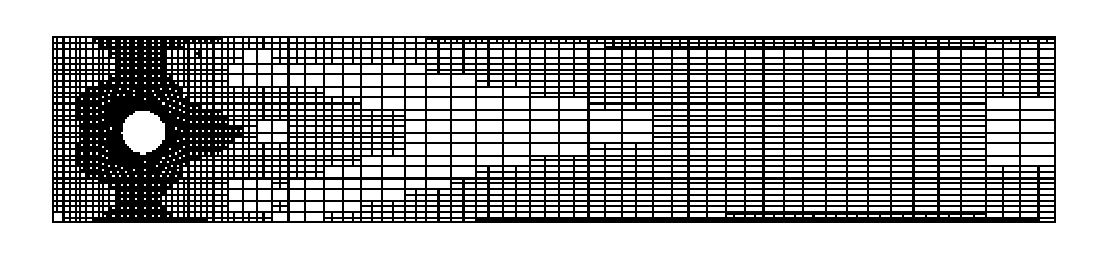
\includegraphics[scale=0.70]{../psfiles/optgrid.eps}
\end{center}
\vspace*{-0.5cm}
\caption{"Optimal grid" via a--posteriori error estimation}
\end{figure}

As can be seen the adaptive grid refinement techniques are needed only locally, near the boundaries, while 
mostly regular substructures (up to 90 \%) can be used in the interior of the domain. 
This is a quite typical result and shows that even for (more or less) complex flow simulations 
(here as a prototypical example) locally blockwise structured meshes can be applied: 
these regions can be detected and exploited by the given hierarchical strategies.

The {\sc ScaRC} approach consists of a separated multigrid approach for every hierarchical
layer, whereby the multigrid scheme on the outest layer (subdomain layer)
gives the final result. The smoothing step of the multigrid method is
based on the following notation:

\vspace*{0.2cm}

{ {Smoothing on level $h$ for $A_h x=b_h$:}}


\begin{itemize}
\item {\bf global} outer block Jacobi scheme (with averaging operator `M')
\[ x^{l+1} = x^l - \omega_g \tilde{A}^{-1}_{h,M} (A_h x^l - b_h) \]
with $\tilde{A}^{-1}_{h,M} := M \circ \tilde{A}^{-1}_{h}$ \,,\,
$\displaystyle \tilde{A}^{-1}_{h} := \sum_{i=1}^N \tilde{A}^{-1}_{h,i}$ \,,\,
$\tilde{A}_{h,i} := "A_{h|\Omega_i}"$

\item "solve" {\bf local} problems $\tilde{A}_{h,i} y_i = def_i^l := (A_h x^l - b_h)_{|\Omega_i}$ via
\[ y_i^{k+1} = y_i^k - \omega_l C^{-1}_{h,i} (\tilde{A}_{h,i} y_i^k - def_i^l) \]
with $C^{-1}_{h,i}$ preconditioner for $\tilde{A}_{h,i}$, or employ a direct solver
\end{itemize}

The local smoothing operators can be a further multigrid scheme
or any other scheme like Jacobi, Gau{\ss}--Seidel, ADI or ILU. The choice of the method depends on the local 
structure and the numerical difficulties caused by the given domain. In a first step this decision is taken by
the user to choose explicitly the method but in future it is possible to use
an "expert system" which makes this decision widely automatically. 

\vspace*{0.2cm}

There are several reasons why we explicitely use {\bf this} {\em basic iteration}:

\begin{enumerate}
\item This general form allows the splitting into matrix--vector 
multiplication, preconditioning and linear combination. All 3 components can be 
separately performed with high performance tools if available.
\item The explicit use of the complete defect $A_h x^l - b_h$ is  advantageous for certain 
techniques for implementing boundary conditions (see \cite{Turek1999h}).
\item All components in standard multigrid, i.e., smoothing, defect calculation, step--length control, 
grid transfer, are included in this {\em basic iteration}.
\end{enumerate}

Figure \ref{scarcscheme} shows an example illustration of a \scarc scheme.

%########################################################
\vspace*{0.5cm}

\begin{figure}[!h]
\hspace*{2cm}\begin{minipage}{7cm}
Standard multigrid with\\
(recursively defined)\\
block smoothers\\

\vspace*{0.2cm}
plus
\vspace*{0.2cm}

Standard Domain Decomposition\\
with minimal overlap,\\
sequence of coarse grid \\
problems via multigrid\\

\vspace*{0.2cm}
plus
\vspace*{0.2cm}

Embedded into \\
standard CG--method\\

\vspace*{-7cm}\hspace*{6cm}\includegraphics[scale=0.45]{../psfiles/groid.ps}
\end{minipage}
\caption{\scarc scheme: example}
\label{scarcscheme}
\end{figure}


%########################################################


The notation \scarc stands for:
\begin{itemize}
\item {\bf Scalable}, w.r.t. the number of global ('$l$') and local solution steps ('$k$'),
\item {\bf Recursive}, since it may be applied to more than 2 global/local levels,
\item {\bf Clustering}, since fixed or \underline{adaptive} blocking of substructures is possible.
\end{itemize}

%########################################################

\begin{figure}[!h]
\begin{center}
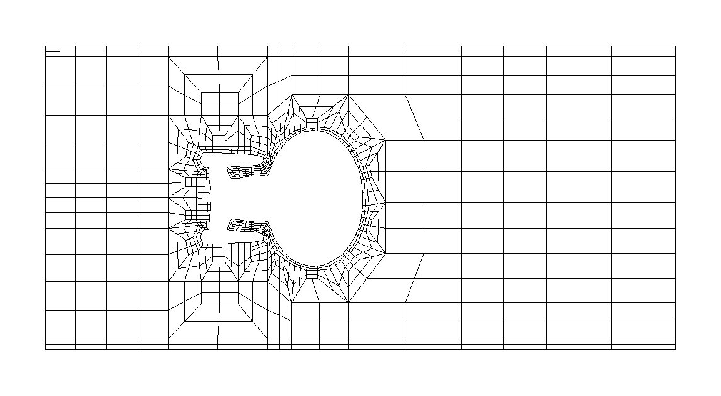
\includegraphics[width=7cm]{../psfiles/gitter1.ps}
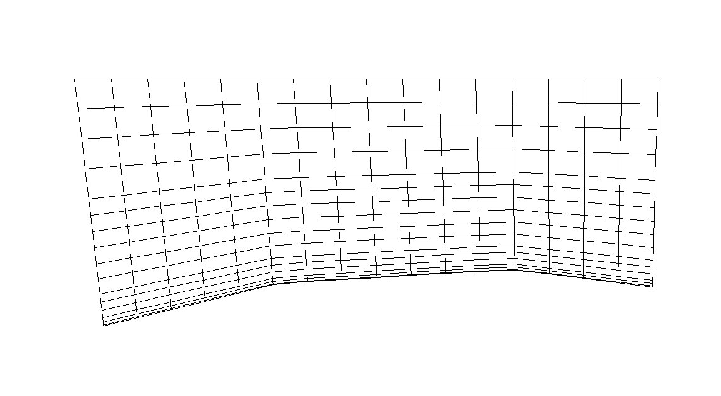
\includegraphics[width=8cm]{../psfiles/makro.ps} 
\end{center}
\caption{Example of ScaRC: 2D decomposition and zoomed (macro) element (LEVEL 3) with locally anisotropic 
refinement towards the wall}
\label{scarcexamplegrid}
\end{figure}

%########################################################

Results for a ScaRC-CG solver (smoothing steps: 1 global ScaRC; 1 local `MG-TriGS') 
for locally (an)isotropic refinement are shown in table \ref{scarcresults}.


\begin{table}[!h]
\begin{center}
\begin{tabular}{|r||c|c|c|c|}
\hline
$\#NEQ$ \phantom{  }        & \multicolumn{2}{c|}{Dirichlet 'Velocity'} & \multicolumn{2}{c|}{Neumann 'Pressure'} \\
\cline{2-5}
& $AR \approx 10$ &  $AR \approx 10^{6}$ & $AR \approx 10$ &  $AR \approx 10^{6}$ \\
\hline \hline
   $210,944$    & 0.17 ({\bf 8}) & 0.18 ({\bf 8}) & 0.21 ({\bf 9}) & 0.15 ({\bf 8}) \\
   $843,776$    & 0.17 ({\bf 8}) & 0.17 ({\bf 8}) & 0.20 ({\bf 9})  & 0.17 ({\bf 8}) \\
   $3,375,104$  & 0.18 ({\bf 9}) & 0.19 ({\bf 9}) & 0.22 ({\bf 10}) & 0.22 ({\bf 10}) \\ 
   $13,500,416$ & 0.19 ({\bf 9}) & 0.18 ({\bf 9}) & 0.23 ({\bf 10}) & 0.23 ({\bf 10}) \\ 
   \hline
\end{tabular}
\end{center}
\caption{Global (parallel) convergence rates for \scarc on configuration shown in \ref{scarcexamplegrid}}
\label{scarcresults}
\end{table}


For
more information about {\sc ScaRC} see \cite{KilianTurek1998} and \cite{Kilian2001}.


\subsection{High Performance Linear Algebra}


One of the main ideas behind the described {\it (Recursive) Divide and Conquer} approach in 
combination with the {\sc ScaRC} solver technology is to detect "locally structured parts". 
In these "local subdomains" we apply consequently "highly structured tools" as known from Finite Difference  
approaches: line-- or rowwise numbering of unknowns and storing of matrices as 
sparse bands (however the matrix entries are calculated via the Finite Element modules). 
As a result we have "optimal" data structures on each of these patches (which often correspond to 
the former introduced "matrix blocks") and we can perform very powerful 
linear algebra tools which explicitly exploit the high performance of specific 
machine optimised libraries.

We have performed several tests for different tasks 
and techniques in numerical linear algebra  on some selected hardware platforms.
In all cases we attempted to use "optimal" compiler options and 
machine optimised linear algebra libraries.

{\bf Matrix--vector multiplication:}

We examine more carefully the following variants which all are typical in the context of 
iterative schemes with sparse matrices. The test matrix is a 
typical 9--point stencil (emerging from a FE discretisation of the Poisson operator with bilinear Finite 
Elements). We perform tests for two different vector lengths $N$ and give the measured MFLOP rates which are all calculated via $20 \times N/time$ (for MV), resp., 
$2 \times N/time$ (for DAXPY). 

{\bf Sparse MV: SMV}\\
The {\em sparse MV} technique (see \ref{sparsematvecmul}) is the standard technique in Finite Element codes (and others), also well known 
as "compact storage" technique or similar: the matrix plus index arrays or lists are stored as long arrays 
containing the nonzero elements only. While this approach can be applied for arbitrary meshes and 
numberings of the unknowns, no explicit advantage of the linewise numbering can be 
exploited. We expect a massive loss of performance with respect to the possible peak rates since --- at least 
for larger problems --- no "caching in" and "pipelining" can be exploited such that the higher cost of 
memory access will dominate the resulting MFLOP rates. Results are shown in table \ref{sparsematvecmulresult}.


%#################################################################

\begin{code}{ Standard sparse matrix vector algorithm(DAXPY indexed)}{sparsematvecmul}
\begin{verbatim}
                             DO 10 IROW=1,N
                             DO 10 ICOL=KLD(IROW),KLD(IROW+1)-1
                     10      Y(IROW)=DA(ICOL)*X(KCOL(ICOL))+Y(IROW)
\end{verbatim}
\end{code}

\begin{table}[!h]
\begin{center}
\begin{tabular}{|c|c||c|c||c|} \hline
Computer     & \#Unknowns  & {\bf CM}&{\bf TL}&{\bf STO}\\ \hline
%
                                           &     8,320 & 147 & 136 & {\bf 116} \\
                                           &    33,280 & 125 & 105 & {\bf 100} \\
{\bf Alpha ES40}                           &   133,120 & 81  & 71 & {\bf 58} \\
(667 Mhz)                                  &   532,480 & 60  & 51 & {\bf  21} \\
                                           & 2,129,920 & 58  & 47 & {\bf  13} \\
                                           & 8,519,680 & 58  & 45 & {\bf  10} \\ \hline
\end{tabular}
\end{center}
\caption{Performance rates of the FEATFLOW code with
different numbering schemes (Cuthill--McKee, TwoLevel, Stochastic)
for matrix vector multiplication}
\label{sparsematvecmulresult}
\end{table}

%#################################################################

{\bf Banded MV: BMV}\\
A "natural" way to improve the {\em sparse MV} is to exploit that the matrix consists of 9 bands only. 
Hence the matrix--vector multiplication is rewritten such that now 
"band after band" are applied.  The obvious advantage of this {\em banded MV} approach is that these tasks can be performed on the basis of BLAS1--like routines which may exploit the vectorisation facilities 
of many processors (particularly on vector computers). However for "long" vector lengths the 
improvements can be absolutely disappointing: For the recent workstation/PC chip technology the processor cache dominates the resulting efficiency!


{\bf Banded blocked MV: BBMVA, BBMVL, BBMVC}\\
The final step towards highly efficient components is to rearrange the matrix--vector multiplication 
in a "blockwise" sense: for a certain set of unknowns, a corresponding part of the matrix is treated 
such that cache--optimised and fully vectorised operations can be performed. This procedure is called 
"BLAS 2+"--style since in fact certain techniques for dense matrices which are based on ideas 
from the BLAS2, resp., BLAS3 library, have now been developed for such sparse banded matrices. 
The exact procedure has to be carefully developed in dependence of the underlying FEM discretisation, 
and a more detailed description can be found in \cite{Becker2003}. 

While BBMVA has to be applied in the case of arbitrary matrix coefficients, BBMVL and BBMVC are 
modified versions which can be used under certain circumstances only (see \cite{Becker2003} for 
technical details). For example PDE's with constant coefficients as the Poisson operator but 
on a mesh which is adapted in one special direction only, allow the use of BBMVL: This is often the case for the 
Pressure--Poisson problem in flow simulations on boundary adapted meshes. 
Additionally version BBMVC may be applied for PDE's with constant coefficients on meshes with equidistant 
mesh distribution in each (local) direction separately: This is typical for tensor product meshes 
in the interior domain where the solution is mostly smooth.

Performance results for banded techniques in comparation to standard techniques are shown in table \ref{sbblasresults1}.

As example the Poisson problem with multigrid with TriGS smoother on NCC-1701D grid is calculated, corresponding
performance results are shown in table \ref{sbblasresults}.

%#################################################################


\begin{table}[!h]
\begin{center}
\begin{tabular}{|c|c|c|c|c|c|c|} \hline
2D case     & N  &{DAXPY(I)}&  \multicolumn{2}{c|}{MV} & \multicolumn{2}{c|}{MG-TriGS} \\ \hline
   &  & & V & C &  V & C \\ \hline
%
{Sun V40z     }    & $65^2$     & 1521 (422)    & 1111     &  1605    & 943      & 1178      \\
{(1800 MHz)     } & $257^2$     &  264 (106)     & 380     &  1214    & 446      & 769      \\
{`{\bf Opteron}'  } &{\bf $1025^2$}&{\bf  197 (54)}&{\bf 362}&{\bf 1140}&{\bf 333} &{\bf 570} \\ \hline

{DEC 21264     } & $65^2$     & 205 (178)    & 538     &  795    & 370      & 452      \\
{(667 MHz)     } & $257^2$     &  224 (110)     & 358     &  1010    & 314      & 487      \\
{`{\bf ES40}'  } &{\bf $1025^2$}&{\bf  78 (11)}&{\bf 158}&{\bf 813}&{\bf 185} &{\bf 401} \\ \hline


{NEC SX-6}   & $65^2$     & 1170 (422)    &1204     &  1354    & 268      & 341      \\
{(500 MHz)} & $257^2$   & 1100 (412)    &1568     &  2509    & 316      & 459      \\
{ `{\bf Vector}'   } &{\bf $1025^2$}&{\bf  1120 (420)}&{\bf 1597}&{\bf 3421}&{\bf 339} &{\bf 554} \\ \hline


{IBM POWER4}           & $65^2$   &1521 (845)    &  2064     &  3612    &  1386     &  1813     \\
{(1700 MHz)     }      & $257^2$   &1100 (227)   &  1140     &  3422    &  1048     &  1645     \\
{`{\bf Power}'}        &{\bf $1025^2$} &{\bf  390 (56)}&{\bf  550}&{\bf 2177}&{\bf  622}&{\bf  1138}\\ \hline
%
\end{tabular}
\end{center}
\caption{Performance rates for the operations DAXPY, DAXPY-I, MV and MG-TriGS for different arhitectures}
\label{sbblasresults1}
\end{table}

%#################################################################

\begin{table}[!h]
\begin{center}
\begin{tabular}{|c|c|c|c|c|} \hline
N         &    1p        &    2p       &     3p      &      4p\\ \hline
843,776    &  11.04(191)  &  5.72(368)  &  3.85(547)  &  3.45 (611) \\ 
3,381,507   &  30.36(271)  &  15.62(526) &  10.73(766) &  8.42 (976) \\
13,513,219  &  98.64(328)  &  51.04(634) &  34.79(931) &  27.80(1165) \\
54,027,267  &  367.85(301) & 198.35(559) &  129.07(859) & 107.70(1029) \\ \hline
\end{tabular}
\end{center}
\caption{CPU times and numerical MFlop rates for different numbers of CPUs
(Sun V40z, four Opteron 844 CPUs with 1800Mhz, 16 GByte memory)}
\label{sbblasresults}
\end{table}


More information in available in \cite{AltieriBeckerTurek1998}, \cite{BeckerKilianTurek1999a} and
\cite{TurekBeckerKilian2003a}.

%#################################################################
As a summary, we can draw the following conclusions:
\begin{itemize}
\item Sparse techniques are the basis for most of the recent
software packages.
\item Different numberings can lead to identical
numerical results and work (w.r.t. arith.ops and data accesses) but
to huge differences in CPU time.
\item Sparse techniques are 'slow'. The computational speed depends on the problem 
size and the kind of data access.
\end{itemize}


\subsection{Several adaptivity concepts}

As typical of modern FEM packages, we directly incorporate certain tools for grid 
generation which allow easy handling of local and global refinement or coarsening strategies:
{\bf adaptive mesh moving}, {\bf macro adaptivity} and {\bf fully local adaptivity}.

Adaptive strategies for moving mesh points, along boundaries or inner structures, allow the same 
logic structure in each "macro block", and hence the shown performance rates can be preserved. 
Additionally, we work with adaptivity concepts related to 
each "macro block". Allowing "blind" or "slave macro nodes" preserves the 
high performance facilities in each "matrix block", and is a good compromise between fully local 
adaptivity and optimal efficiency through structured data. Only in that case, that these concepts do not 
lead to satisfying results, certain macros will loose their "highly structured" features through 
the (local) use of fully adaptive techniques. On these (hopefully) few patches, the standard "sparse" 
techniques for unstructured meshes have to be applied.

\subsection{Direct integration of parallelism}

Most software packages are designed for sequential algorithms to solve a given PDE problem, and the 
subsequent parallelisation of certain methods takes often unproportionately long. 
In fact it is easy to say, but hard to realise with most software packages.  However the more important step, which makes parallelisation 
much more easier, is the design of the {\sc ScaRC} solver according to the hierarchical decomposition 
in different stages. Indeed from an algorithmic point of view, our sequential and parallel 
versions differ only as analogously Jacobi-- and Gau{\ss}--Seidel--like schemes work differently. 
Hence all parallel executions can be identically simulated on single processors which however can 
additionally improve their numerical behaviour with respect to efficiency and robustness through 
Gau{\ss}--Seidel--like mechanisms. 

Hence we only provide in {\sc FEAST} the "software" tools for including parallelism on low 
level, while the "numerical parallelism" is incorporated via our {\sc ScaRC} solver and the 
hierarchical "tree structure". However what will be "non--standard" is our concept of (adaptive) 
parallel loadbalancing 
which is oriented in "total numerical efficiency" (that means, "how much processor work is spent to achieve 
a certain accuracy, depending on the local configuration") in contrast to the "classical" criterion of 
equilibrating the number of local unknowns (see \cite{Becker2003} for detailed information and examples in {\sc FEAST}).

\section{Pre-- and Postprocessing}

\subsection{General remarks}
%
As remarked in the introduction the pre-- and postprocessing should
be realised in main tasks by a general framework of Java based programs 
called DeViSoR. DeViSoR means "Design \& Visualisation Software Resource".
This framework is intented to perform the main tasks grid generation and
editing, control of the calculation and visualisation of the results. 
These main tasks use the same ground classes (called DFC - DeViSoR Foundation
Classes) and the same user interface, so the access to the underlying 
numerical core parts are  performed in the same manner.

As intented in the introduction the various subtasks can be performed on
several machines which communicates over a network system. This allows
the user to choose the suitable system for the corresponding task, e.g.
a Silicon Graphics workstation for the visualisation. The access to
a parallel computing system should also be performed by a Java program.
This allows not only the developer of a numerical code to use a
parallel computer.

DeViSoR is planned to be an "open system" for the developing of pre-- and
postprocessing tools for FEM packages. The DeViSoR foundation classes
contain the basic tools to handle and administrate FEM typical structures.
Further applications could realise e.g. further visualisation procedures
and adaptions to several parallel computer systems.

For this project Java as implementation environment is been choosen. Though Java
is a relative "young" programming language the advantages of this system
are significant. The "write once, run anywhere" capability reduces the
implementation effort widely against combinations like C/C++/OpenGL. It
exist only one program which runs without any modification on several
different configurations like Unix workstations, Linux PCs, Windows PCs,
Macintoshs and many more. A further advantage is the core
class library for various subareas like file hand\-ling, network functions,
visualisation and user interface facilities. These classes are easy to use and
produce an pleasing output. The use of additional tools like applications
builders is not necessary. The most disadvantage of nowadays Java
implementations is the relative low performance because of the fact that
Java is an interpreted language.  However further developments like
more sophisticated interpreter with Just--In--Time compiling facilities and
especially the native Java processor will hopefully close this 
performance leak.

More information you can find in \cite{PGDeViSoR2003}.

\subsection{Preprocessing: DeViSoRGrid}

This subprogram should support the generation and editing of 2D domains.
The two main parts are the description of the domain boundary and the 
generation of the grid structure. The program supports several boundary
elements like lines, arcs and splines, further it is planned to add a
segment which consists of an Fortran subroutine which describes a
parametrisation. This allows to use an analytic description. 
Several triangular and quadrilateral elements
are supported. Extensive editing possibilities allow the user to delete, move
and adjust the boundaries and elements. For the future it is planned to implement simply automatic grid generators
for producing coarse grids. As further tasks this program should be able to read many formats from
other tools like CAD systems and professional grid generators and prepare
this data for the use in the calculation process.

\subsection{Processing: DeViSoRControl}

DeViSoRControl enables the user to control the calculation und to follow the
calculation progress. Main tasks of this program part are the distribution
of the macros to the processing nodes (at the moment manually, in future
automa\-tically), the collecting and displaying of the log information of the
processing nodes and finally the configuration of the {\sc ScaRC} algorithm with
respect to the selection of smoothing/preconditioning methods on a given
hierarchical layer, the size of smoothing steps and the stopping criterion.
Furthermore this part builds the interface to the other DeViSoR parts for
the pre-- and postprocessing. From the control part the grid program is
invoked, a grid is editing. For this grid the user selects the desired
solution method and visualise finally the results with the DeViSoRVision
program.


\subsection{Postprocessing: DeViSoRVision}

The last part in the current project is the DeViSoRVision program which
performs the visualisation task. The program offers several techniques to
visualise the results of the calculation like shading techniques, isolines,
particle tracing (planned). Furthermore it contains an animation module to
create animations for nonstationary problems. The result of the animation
can be stored in several formats like MPEG and AnimatedGIF. 

